\documentclass[a4paper]{article}
\usepackage[german,english]{babel}
\usepackage{amsmath}
\usepackage{amssymb}
\usepackage{amsthm}
\usepackage{graphicx}
\usepackage{caption}
\usepackage{centernot}
\usepackage{fontspec}
\usepackage{mdframed}
\usepackage{pxfonts}
\usepackage{wasysym}
\usepackage{framed}
\usepackage{xcolor}
\usepackage{makeidx}
\usepackage{csquotes}
\usepackage[pdfborder={0 0 0}]{hyperref}
\usepackage{stmaryrd}
\usepackage{unicode-math}
\usepackage{titlesec}
\titleformat{\paragraph}{\normalfont\itshape}{}{}{}

% okay-ish main typefaces: Alegreya, Junicode, CMU Concrete, Linux Libertine O, Libertinus Serif, URW Palladio L, Bookerly, Andada
\setmainfont{Alegreya}  % TODO \setminus is broken, \textbackslash{} is used instead
\setmathfont{cmr10}


\newcounter{lecref}[section]
\numberwithin{lecref}{section}

\theoremstyle{break}
\newmdtheoremenv[
    linecolor=white,%
    backgroundcolor=gray!10,%
    innertopmargin=0pt]{theorem}{Theorem}[lecref]

%\newtheorem{theorem}[lecref]{Theorem}
\newtheorem*{Theorem}{Theorem}
\newtheorem{example}[lecref]{Example}
\newtheorem*{Example}{Example}
\newtheorem{definition}[lecref]{Definition}
\newtheorem*{Definition}{Definition}
\newtheorem{lemma}[lecref]{Lemma}
\newtheorem*{Lemma}{Lemma}
\newtheorem{claim}[lecref]{Claim}
\newtheorem*{Claim}{Claim}
\newtheorem{remark}[lecref]{Remark}
\newtheorem*{Remark}{Remark}
\newtheorem{algorithm}[lecref]{Algorithm}
\newtheorem*{Algorithm}{Algorithm}
\newtheorem{corollary}[lecref]{Corollary}
\newtheorem*{Corollary}{Corollary}
\newtheorem{proposition}[lecref]{Proposition}
\newtheorem*{Proposition}{Proposition}


\def\ifempty#1{\def\temp{#1} \ifx\temp\empty }

% chronological structure of lectures
\newcommand{\dateref}[1]{%
  \begin{mdframed}[backgroundcolor=gray!10,innerbottommargin=0pt,innertopmargin=0pt]
    \paragraph{\textit{$\downarrow$ This lecture took place on #1.}}%
  \end{mdframed}%
}

% useful control sequences for mathematical notation
\newcommand{\Abs}[1]{\left|#1\right|}
\newcommand{\Set}[1]{\left\{#1\right\}}
\newcommand{\SetDef}[2]{\left\{#1\,\mid\,#2\right\}}
\newcommand{\IP}[2]{\left\langle#1, #2\right\rangle}
\newcommand{\Norm}[1]{\left\|{\ifempty{#1}\cdot\else#1\fi}\right\|}
\newcommand{\Max}[1]{\max{\Set{#1}}}
\newcommand{\Min}[1]{\min{\Set{#1}}}
\newcommand{\Sup}[1]{\sup{\Set{#1}}}
\newcommand{\Powerset}[1]{{\mathbb P}(#1)}
\newcommand{\IntRange}[2]{#1, \dots\ifempty{#2}\else, #2\fi}

\def\vec2#1#2{\begin{pmatrix} #1 \\ #2 \end{pmatrix}}
\def\vec3#1#2#3{\begin{pmatrix} #1 \\ #2 \\ #3 \end{pmatrix}}
\newcommand{\noproof}[1]{A proof for Theorem~\ref{#1} is not provided.}
\newcommand{\dotted}[1]{\:\dot{#1}\:}  % dot has too little margin

% German translation
\newcommand{\dt}[1]{(dt. \enquote{\foreignlanguage{german}{#1}})}

% essential control sequences
%% \xRightarrow: \xrightarrow for \rightarrow like \xRightarrow for \Rightarrow
\makeatletter
\newcommand{\xRightarrow}[2][]{\ext@arrow 0359\Rightarrowfill@{#1}{#2}}
\makeatother


\makeatletter
\def\moverlay{\mathpalette\mov@rlay}
\def\mov@rlay#1#2{\leavevmode\vtop{%
   \baselineskip\z@skip \lineskiplimit-\maxdimen
   \ialign{\hfil$\m@th#1##$\hfil\cr#2\crcr}}}
\newcommand{\charfusion}[3][\mathord]{
    #1{\ifx#1\mathop\vphantom{#2}\fi
        \mathpalette\mov@rlay{#2\cr#3}
      }
    \ifx#1\mathop\expandafter\displaylimits\fi}
\makeatother

\newcommand{\cupdot}{\charfusion[\mathbin]{\cup}{\cdot}}
\newcommand{\bigcupdot}{\charfusion[\mathop]{\bigcup}{\cdot}}


% typesetting settings
\parindent0pt
\setlength{\parskip}{.6em}

\DeclareMathOperator{\rank}{rank}
\DeclareMathOperator{\diag}{diag}
\DeclareMathOperator{\detm}{det}
\DeclareMathOperator{\perm}{perm}
\DeclareMathOperator{\sign}{sign}
\DeclareMathOperator{\degree}{deg}
\DeclareMathOperator{\im}{image}
\DeclareMathOperator{\ke}{kernel}
\DeclareMathOperator{\prop}{probability}
\DeclareMathOperator{\Hom}{Hom}
\DeclareMathOperator{\argmax}{argmax}
\DeclareMathOperator{\argmin}{argmin}
\DeclareMathOperator{\vol}{vol}  % volume
\DeclareMathOperator*{\bigtimes}{\vartimes}

% https://tex.stackexchange.com/a/110981, CC BY-SA
\makeatletter
\providecommand*{\dotcup}{%
  \mathbin{%
    \mathpalette\@dotcup{}%
  }%
}
\newcommand*{\@dotcup}[2]{%
  \ooalign{%
    $\m@th#1\cup$\cr
    \hidewidth$\m@th#1\cdot$\hidewidth
  }%
}
\makeatother

% metadata
\title{
  Measure and integration theory \\
  \large{Lecture notes, University (of Technology) Graz} \\
  based on the lecture by Wolfgang W\"oss
}
\date{\today}
\author{Lukas Prokop}

% generate index database
\makeindex


\begin{document}
\newcommand\gen{{\mathcal E}}
\renewcommand\setminus{\,{\textbackslash{}}\,} % TODO interesting: if we put this before begin{document}, it won't take effect

\maketitle
\tableofcontents

\section{Course}

\begin{enumerate}
  \item Thursday, 16:15--18:00
  \item Monday, 12:15--14:00
  \item Exam: oral, date negotiation per email, 3 examinees at once
  \item In this document, $\subset$ denotes $\subseteq$ or $\subsetneq$
  \item Literature: \enquote{Measure Theory} by Paul R. Halmos
\end{enumerate}

\dateref{2018/10/01}

\section{Sigma algebras and measures}

A measure represents the content of a set. In $R^2$, it represents the area. In $R^3$, it represents the volume. In $R^d$, we can consider the content of a subspace as dimensionwise combination of intervals:

\[ [a_1, b_1] \times \dots \times [a_d, b_d] \]

To determine the \enquote{size} of this space, we can use the product of the individual interval sizes:
\[ (b_1 - a_1) \cdot \dots \cdot (b_d - a_d) \]

Consider an geometric object as in Figure~\ref{img:jordan}.
We can approximate the size of $B$ by considering inner or outer axis-parallel boundary.
The approximation using the infimum of the outer and supremum of the inner boundary defines the Jordan measure.

The indicator function of this area ($1_B$) is Riemann-integrable.

\begin{figure}[!ht]
  \begin{center}
    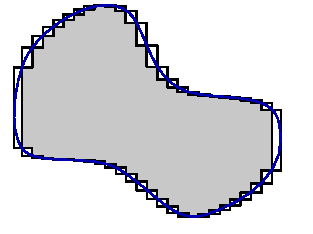
\includegraphics{img/01_jordan-measure.pdf}
    \caption{Jordan measurability of this area $B$}
    \label{img:jordan}
  \end{center}
\end{figure}

A one-point set is Jordan measurable with measure/content $0$. However, $\mathbb Q \cap [0, 1]$ is not Jordan measurable, because the indicator function is not Riemann integrable. It is desirable that the measure $\bigcupdot_{n=1}^\infty A_n = \sum_{n=1}^\infty \operatorname{measure}(A_n)$ (using pairwise disjoint union) holds true.

Modern measure theory was established by Lebesgue (1901):
\begin{enumerate}
  \item Union of countable sets ($\sigma$-additivity)
  \item arbitrary base set $\chi$ instead of $\mathbb R^d$, integration theory for $f: \chi \to \mathbb R$
\end{enumerate}

\subsection{Definition}

\index{Sigma-algebra}
Let $(\delta, \rho)$ be the non-empty base set.
$\mathcal A \subset P(\chi)$. A set system of subsets of $\chi$ is called \emph{sigma-algebra} ($\sigma$-algebra) if
\begin{enumerate}
  \item $\chi \in \mathcal A$
  \item $A \in \mathcal A \implies A^C = \chi \setminus A \in \mathcal A$
  \item $A_n \in \mathcal A$ ($n \in \mathbb N$) $\implies \bigcup_{n=1}^\infty A_n \in \mathcal A$
\end{enumerate}

Properties 1 and 2 implies that $\emptyset \in \mathcal A$.

\index{Measurable space}
\index{Measure}
A \emph{measurable space} is given by $(\chi, \mathcal A)$. A \emph{measure} $\mu: \mathcal A \to [0, \infty]$ is defined by
\begin{enumerate}
  \item $\mu(\emptyset) = 0$
  \item If $A_n \in \mathcal A$ ($n \in \mathbb N$), pairwise disjoint, then
    \[ \implies \mu\left(\bigcup_{n=1}^\infty A_n\right) = \sum_{n=1}^\infty \mu(A_n) \]
\end{enumerate}
\index{Measure space}
A \emph{measure space} is given with $(\chi, \mathcal A, \mu)$.

\begin{Remark}
  \begin{itemize}
    \item $\mu$ is called probability space if $\mu(\chi) = 1$
    \item $\mu$ is called finite measure if $\mu(\chi) < \infty$
    \item $\mu$ is called $\sigma$-finite if $\chi = \bigcup_{n=1}^\infty A_n$ with $A_n \in \mathcal A$ and $\mu(A_n) < \infty$ (e.g. real axes decomposes into intervals of length $1$)
  \end{itemize}
\end{Remark}

Examples:
\begin{enumerate}
  \item $\chi$ is at most countable, then mostly $\mathcal A = \Powerset{\chi}$.
    Then it suffices to know, $\mu(\Set{x}) \in [0, \infty)$.
    Then we denote $\mu(x) = \mu(\Set{x})$ with $x \in \chi$.
    \[ \mu(A) = \sum_{x \in A} \mu(x) \]
    e.g. $\mu(x) = 1 \forall x \in \chi$ in case of a \emph{counting measure}.
    \index{Counting measure}
  \item If $\chi$ is uncountable, e.g. $\mathbb R^d$, then it is not recommended to use $\Powerset{\chi}$. So what about $A$? Consider for example $\mathbb R^d$. All $[a_1, b_1] \times \dots \times [a_d, b_d]$ should be elements of $\mathcal A$
\end{enumerate}

\subsection{Simple properties of sigma-algebras}

\begin{enumerate}
  \item $\emptyset \in \mathcal A$
  \item $A_1, \dots, A_n \in \mathcal A \implies \bigcup_{k=1}^n A_k \in \mathcal A$
  \item $A_n \in \mathcal A$ ($n \in \mathbb N$) or $\IntRange{}{N} \implies \bigcap_{n \in \mathbb N} A_n \in \mathcal A$ (deMorgan) $\bigcap_{n} A_n = \left(\bigcup_n A_n^C\right)^C$
  \item $A, B \in \mathcal A \implies A \setminus B \in \mathcal A$, $A \triangle B = A \setminus B \lor B \setminus A$
\end{enumerate}

\index{Generating set}
\index{Generator}
\begin{definition}[Generating set]
  Let $\gen \neq \emptyset$ with $\gen \subset \Powerset{\chi}$ be the \emph{generator} (generating set) of the $\sigma$-algebra. $\sigma(\gen)$ is the smallest $\sigma$-algebra over $\chi$ which contains $\gen$.
  \[
    = \bigcap \Set{
      \tilde A: \tilde A \text{ is the } \sigma-\text{algebra over } \chi \text{ with } \gen \subset \tilde{\mathcal A}
    }
  \]
  This set is non-empty because $\Powerset{\chi}$ is the $\sigma$-algebra for all $\chi$ and $\gen \subset \Powerset{\chi}$
\end{definition}

\begin{lemma}
  If $\mathcal A_i$ with $i \in I$ is a family of $\sigma$-algebras,
  then $\bigcap_{i \in I} \mathcal A_i$ is a $\sigma$-algebra over $\chi$.
\end{lemma}

Immediate:
\begin{enumerate}
  \item if $\gen_1 \subset \gen_2$ ($\implies \gen_1 \subset \sigma(\gen_2)$), then $\sigma(\gen_1) \subset \sigma(\gen_2)$
  \item if additionally $\gen_2 \subset \sigma(\gen_1)$, then $\sigma(\gen_1) = \sigma(\gen_2)$
\end{enumerate}

Example:
\[ \chi = \bigcup_{n \in I} E_n \neq \emptyset \qquad I = \mathbb N \text{ or } \{\IntRange1N\} \]
\[ \gen = \SetDef{E_n}{n \in I} \qquad \sigma(\gen) = \SetDef{\bigcup_{n \in J} E_n}{J \subset I} \]
\begin{enumerate}
  \item Is a $\sigma$-algebra
  \item If $\gen \subset \tilde{\mathcal A}$, then $\SetDef{\bigcup_{n \in J} E_n}{J \subset I} \subset \tilde{\mathcal A}$
\end{enumerate}

\begin{Definition}
  $(\chi, d)$ is a metric space.
  Borel-$\sigma$-algebra $\sigma(\mathcal O)$.
  $\mathcal O$ is the set of open sets in a metric space
\end{Definition}

\begin{Example}
  Consider $\mathbb R^d$. $\mathcal B_{\mathbb R^d}$ denotes the Borel $\sigma$-algebra.
  \begin{enumerate}
    \item $\gen_1 = \Set{\text{open sets}}$
    \item $\gen_2 = \Set{\text{closed sets}}$
    \item $\gen_3 = \Set{(a_1, b_1) \times \dots \times (a_d, b_d): a_i, b_i \in \mathbb R, a_i < b_i}$ is a parallelepiped
    \item $\sigma(\gen_1) = \sigma(\gen_2) = \sigma(\gen_3) = \mathcal B_{\mathbb R^d}$
    \item $\sigma(\gen_3) = \mathcal B_{\mathbb R^d}$ because every open set is a countable union of open (or left half-open) parallelepipeds
  \end{enumerate}
\end{Example}
\[ \gen_3 \subset \gen_1 \subset \sigma(\gen_3) \]
\[ \gen_4 = \SetDef{(a_1, b_1] \times \dots \times (a_d, b_d]}{a_i, b_i \in \mathbb R, a_i < b_i} \]
\[ (a, b) = \bigcup_{n=1}^\infty (a, b - \frac1n] \]
\[ \gen_5 = \SetDef{(-\infty, b_1) \times \dots \times (-\infty, b_d]}{b_i \in \mathbb R} \text{ because } \gen_4 \subset \sigma(\gen_5) \]
If $d=1$, $(a, b] = (-\infty, b] \setminus (-\infty, a]$. Recognize that $A \setminus B = (A \cap B^C)$. \\
If $d=2$,
\[ (a_1, b_1] \times (a_2, b_2] = (-\infty, b_1] \times (-\infty, b_2] \setminus (-\infty, a_1] \times (-\infty, b_2) \setminus (-\infty, b_1] \times (-\infty, a_2] \]

\index{Trace $\sigma$-algebra}
\begin{Definition}
  $(\chi, \mathcal A)$ is a measurable space, $B \in \mathbb A$ is a trace $\sigma$-algebra over $B$. $\SetDef{A \in \mathcal A}{A \subset B}$
\end{Definition}

\index{Measurable maps}
\begin{Definition}
  $\varphi: (\chi_1, \mathcal A_1) \to (\chi_2, \mathcal A_2)$ is called measurable
  $\iff \varphi^{-1}(A_2) \in \mathcal A_1 \forall A_2 \in \mathcal A_2$
\end{Definition}

\begin{Remark}
  In general $\varphi$ is a map from $\chi_1$ to $\chi_2$.
  $\mathcal A_1$ and $\mathcal A_2$ are mentioned to clarify that the map depends on the chosen algebra.
\end{Remark}

\begin{Remark}
  $(\chi_1, d_1) \to (\chi_1, d_2)$ on metric spaces is continuous iff $\varphi^{-1}(O_2) \in \mathcal O_1 \forall O_2 \in \mathcal O_2$ where $\mathcal O_1, \mathcal O_2$ are sets of open sets.
\end{Remark}

\begin{Remark}
  Measurable maps are a much stronger statement than continuity, because they cover much more sets than open ones.
\end{Remark}

\begin{lemma}
  The composition of measurable maps is measurable.
  \[ \varphi: (\chi_1, \mathcal A_1) \to (\chi_2, \mathcal A_2) \text{ measurable} \]
  \[ \psi: (\chi_2, \mathcal A_2) \to (\chi_2, \mathcal A_2) \text{ measurable} \]
  \[ \implies \psi \circ \varphi: (\chi_1, \mathcal A_1) \to (\chi_3, \mathcal A_3) \text{ measurable} \]
\end{lemma}
\begin{proof}
  Show that $(\psi \circ \varphi)^{-1} (\mathcal A_3) \in \mathcal A_1$ is trivial.
\end{proof}

\begin{theorem}
  Let $\gen_2$ be a generator of $\mathcal A_2$. Then $\varphi: (\chi_1, \mathcal A_1) \to \chi_2$ is measurable in regards of $\mathcal A_2$ iff $\varphi^{-1}(E_2) \in \mathcal A_1 \forall E_2 \in \gen_2$
\end{theorem}
\begin{proof}
  \begin{description}
    \item[$\implies$] is immediate
    \item[$\impliedby$] $\tilde{\mathcal A_2} = \SetDef{A_2 \in \mathcal A_2}{\varphi^{-1}(A_2) \in \mathcal A_1}$ is a $\sigma$-algebra over $\chi_2$. $\gen_2$ is a TM of this $\sigma$ algebra.
    \[ \implies \mathcal A_2 = \sigma(\gen_2) \subset {\tilde{\mathcal A}}_2 \]
  \end{description}
\end{proof}

\begin{example}
  $f: \mathbb R \to \mathbb R$ is monotonically increasing
  \[ f^{-1}(-\infty,b] = \SetDef{x}{f(x) \leq b} = (-\infty, c) \in \mathcal B \]
  Thus, $f$ is measurable.
\end{example}

\begin{Remark}
  $\overline{\mathbb R} \coloneqq \mathbb R \cup \Set{-\infty, +\infty}$
\end{Remark}

\begin{example} \hfill{}
  \[ \mathcal B_{\overline{\mathbb R}} = \SetDef{B, B \cup \Set{-\infty}, B \cup \Set{+\infty}, B \cup \Set{+\infty, -\infty}}{B \in \mathcal B_{\mathbb R}} \]
  $f_1, \dots, f_n: \mathbb R \to \overline{\mathbb R}$ measurable in $(\chi, \mathcal A)$ and $f = \Max{f_1, \dots, f_n}$
  \[ f: \mathbb R \to \overline{\mathbb R} \qquad x \mapsto \max\Set{f_1(x), \dots, f_n(x)} \]
  \begin{align*}
    f^{-1}([-\infty, b]) &= \SetDef{x}{f(x) \leq b} \\
      &= \SetDef{x}{f_k(x) \leq b, k = 1, \dots, n} \\
      &= \bigcap_{k=1}^n \SetDef{x}{f_k(x) \leq b} \in \mathcal B
  \end{align*}
  Analogously for the minimum.
  Therefore $f$ is measurable.
\end{example}

\begin{example}
  The same applies to countably many functions.
  Let $f_n: \mathbb R \to \overline{\mathbb R}$ be measurable with $n \in \mathbb N$.
  Then $f: \sup\SetDef{f_n}{n \in \mathbb N}$ is measurable.
  \begin{align*}
    f^{-1}([-\infty, b]) &= \SetDef{x}{\sup\Set{f_n(x)} \leq b} = \SetDef{x}{f_n(x) \leq b \forall n} \\
      &= \bigcap_{n=1}^\infty \underbrace{f_n^{-1} [-\infty, b]}_{\in B} \in \mathcal B
  \end{align*}
  Analogously for the infimum.
\end{example}

\begin{example}
  \[ \limsup_{n\to\infty} \sup{f_n} = \inf_n \underbrace{\sup_{k \geq n} f_k}_{\text{ with } n\to\infty \text{ monotonically decreasing}} \text{ is measurable} \]
  \[ \liminf_{n\to\infty} f_n = \sup_n \inf_{k \geq n} f_k \text{ is measurable} \]
  if all $f_k$ are measurable. Especially if $f_n \to f$ pointwise and all $f_n$ are measurable, then $f$ is measurable.
\end{example}

\begin{theorem}[Result from the previous example]
  \[ f_n: (\chi, \mathcal A) \to \overline{\mathbb R} \text{ measurable}, n \in \mathbb N \]
  \[ \implies \inf{f_n}, \sup{f_n}, \lim_{n\to\infty} \inf{f_n}, \lim_{n\to\infty} \sup{f_n} \]
  are all measurable.
\end{theorem}

% TODO: this lecture was repetitive, right?

\dateref{2018/10/04}

\begin{enumerate}
  \item Basic set $\chi$ [$\delta, \rho$, \dots]
  \item $\sigma$-algebra $\mathcal A \subset p(\chi)$
    \begin{enumerate}
      \item $\chi \in \mathcal A$
      \item $A \in \mathcal A \implies \mathcal A^C \in \mathcal A$
      \item $A_n \in \mathcal A$ ($n \in \mathbb N$) $\implies \bigcup_{n=1}^\infty A_n \in \mathcal A$
    \end{enumerate}
    $(\chi, \mathcal A)$ is a measurable space
  \item measure $\mu: \mathcal A \to [0, \infty]$
    \begin{enumerate}
      \item $\mu(\emptyset) = 0$
      \item $A_n \in \mathcal A$ ($n \in \mathbb N$), $A_n \cap A_m \neq 0 \forall n \neq m$
        \[ \implies \mu\left(\bigcup_{n=1}^\infty A_n\right) = \sum_{n=1}^\infty \mu(A_n) \qquad \sigma-\text{additivity} \]
        $(\chi, \mathcal A, \mu)$ is a measure space
    \end{enumerate}
  \item ${\mathcal E} \subset p(\chi)$
    \[ \sigma({\mathcal E}) = \bigcap \Set{\tilde A: \tilde A \sigma-\text{algebra}, {\mathcal E} \subset \tilde{A}} \]
    is the so-called ${\mathcal E}$-generated $\sigma$-algebra.
\end{enumerate}
Recognize that ${\mathcal E}_1 \subset {\mathcal E}_2 \implies \sigma({\mathcal E}_1) \subset \sigma({\mathcal E}_2)$.
If additionally, ${\mathcal E}_2 \subset \sigma({\mathcal E}_1) \implies \sigma({\mathcal E}_1) = \sigma({\mathcal E}_2)$.

If $X$ is a metric space, we commonly (sometimes implicitly) use the Borel-Sigma algebra as measure space.

\textbf{Example:}
Let $\mathbb R^d$. Then $\mathcal B_{\mathbb R^d}$ denotes the Borel-sigma algebra.

Let ${\mathcal E}_1$ be the set of open sets. Let ${\mathcal E}_2$ be the set of closed sets.
Let ${\mathcal E}_3 = \Set{(a_1, b_1) \times \dots \times (a_d, b_d): a_i, b_i \in \mathbb R, a_i < b_i}$.
$\sigma(\mathcal E_3) = \mathcal B_{\mathbb R^d}$ because every open set is a countable union of open (or left half-open) parallelepipeds (why countable?).
\[ \mathcal E_3 \subset \mathcal E_1 \subset \sigma(\mathcal E_3) \]

\[ \mathcal E_4 = \Set{(a_1, b_1] \times (a_2, b_2] \times \dots \times (a_d, b_d]} \]
\[ (a, b) = \bigcup_{n=0}^\infty (a, b - \frac1n) \]

\[ \mathcal E_5 = \Set{(-\infty, b_1) \times (-\sigma, b_d): b_1, \dots, b_d \in \mathbb R} \]
because $\mathcal E_4 \subset \sigma(\mathcal E_5)$.

DeMorgan: $A \setminus B = A \cap B^C$

Let $d = 1$, $(a, b] = (-\infty, b] \setminus (-\infty, a]$. \\
Let $d = 2$, $(a_1, b_1] \times (a_2, b_2] = (-\infty, b_1] \times (-\infty, b_2] \setminus (-\infty, a_1] \times (-\infty, b_2] \setminus (-\infty, b_2] \times (-\infty, a_1]$.

\index{Trace $\sigma$-algebra}
\begin{definition}
  Let $(\chi, \mathcal A)$ be a measure space. $B \in \mathcal A$.
  trace $\sigma$-algebra over $B$ is defined as $\Set{A \in \mathcal A: A \subset B}$.
\end{definition}

\begin{Remark}[Revision on continuity]
  Let $\varphi: (\chi_1, d_1) \to (\chi_2, d_2)$ be a map between metric spaces.
  Let $\varphi$ be continuous.

  On the one hand, we know the $\varepsilon$-$\delta$ definition,
  but we also consider $\varphi^{-1}(O_2) \in \mathcal O_1 \forall O_2 \in \mathcal O_2$ (set of open sets)
\end{Remark}

\begin{definition}[Measurable maps]
  Let $\varphi: (\chi_1, \mathcal A_1) \to (\chi_2, \mathcal A_2)$\footnote{Actually, $\varphi: \chi_1 \to \chi_2$, but we don't want to forget about the associated $\sigma$-algebras}
  \[ \iff \varphi^{-1}(A_2) \in \mathcal A_1 \forall A_2 \in \mathcal A_2 \]
\end{definition}

\begin{lemma}
  \label{lem1}
  The composition of measurable maps is measurable.
  \[ \varphi: (\chi_1, \mathcal A_1) \to (\chi_2, \mathcal A_2) \]
  \[ \Psi: (\chi_2, \mathcal A_2) \to (\chi_3, \mathcal A_3) \]
  with $\varphi$ and $\Psi$ measurable.
  \[ \implies \Psi \circ \varphi: (\chi_1, \mathcal A_1) \to (\chi_3, \mathcal A_3) \]
  is measurable. (trivial to prove)
\end{lemma}

\begin{theorem}
  Let $\mathcal E_2$ be the generator of some algebra $\mathcal A_2$.
  Then $\varphi: (\chi_1, \mathcal A_1) \to \chi_2$ in regards of $\mathcal A_2$ is measurable
  if and only if $\varphi^{-1}(E_2) \in \mathcal A_1 \forall E_2 \in \mathcal E_2$.
\end{theorem}
\begin{proof}
  \begin{description}
    \item[$\implies$] trivial
    \item[$\impliedby$]
      $\tilde A_2 \coloneqq \Set{A_2 \in \mathcal A_2: \varphi^{-1}(A_2) \in \mathcal A_1}$
      is a $\sigma$-algebra over $\chi_2$ (why? left as an exercise).
      $\mathcal E_2$ is a subset of this $\sigma$-algebra.
      $\implies \mathcal A_2 = \sigma(\mathcal E_2) \in \tilde A_2 \subset \mathcal A_2$
  \end{description}
\end{proof}

\begin{Example}
  $f: \mathbb R \to \mathbb R$ is monotonically increasing.
  $f^{-1}(-\infty, b] = \Set{x: f(x) \leq b}$ is in the Borel-sigma algebra $\mathcal B$.
  So $f$ is measurable.
\end{Example}

\begin{Definition}
  $\overline{\mathbb R} \coloneqq \mathbb R \cup \Set{-\infty, +\infty}$ \\
  ${\mathcal B}_{\overline{\mathbb R}} = \Set{B, B \cup \Set{-\infty}, B \cup \Set{+\infty}, B \cup \Set{\pm\infty}: B \in \mathcal B_{\mathbb R}}$
\end{Definition}

\begin{example}
  Let $f_1, \dots, f_n: \mathbb R \to \overline{\mathbb R}$ measurable.
  $f = \Max{f_1, \dots, f_n}$.
  \[ f^{-1}([-\infty, b]) = \Set{x: f(x) \leq b} = \Set{x: f_k(x) \leq b, k = 1, \dots, n} = \bigcap_{k=1}^n \underbrace{\Set{x: f_k(x) \leq b}}_{f_k^{-1}[-\infty, b]} \in \mathcal B \]
  Equivalently, $\Min{f_1, \dots, f_n}$ is measurable.
  Equivalently, $f_n: \mathbb R \to \overline{\mathbb R}$ is measurable ($n \in \mathbb N$).
  $\implies f = \Sup{f_n: n \in \mathbb N}$ is measurable.
  \begin{align*}
    f^{-1}(\infty, b] &= \Set{x: \sup f_n(x) \leq b} = \Set{x: f_n(x) \leq b \forall n} \\
    f^{-1}[-\infty, b) &= \Set{x: \sup{f_n(x)} < b} \subset \Set{x: f_n(x) < b \forall n}
  \end{align*}
  \[ \bigcap_{n=1}^\infty \underbrace{f_n^{-1}[-\infty, b]}_{\in \mathcal B} \in \mathcal B \]
\end{example}

Let $f_n$ be measurable functions.
\[ \limsup_{n\to\infty} f_n = \inf_n \sup_{k \geq n} f_k \]
The supremum of measurable functions is measurable (see Lemma~\ref{lem1}). The infimum as well. So the result is measurable.
\[ \liminf_{n\to\infty} f_n = \sup_n \inf_{k \geq n} f_k \]
Equivalently, the result is measurable.

Especially, if $f_n \to f$ pointwise, and all $f_n$ are measurable, then also limit $f$ is measurable.

How to determine measurability? Show that pre-images of generators are in the $\sigma$-algebra.

\begin{theorem}
  Let $f: (\chi, \mathcal A) \to \overline{\mathbb R}$ be measurable ($n \in \mathbb N$)
  \[ \implies \inf{f_n}, \sup{f_n}, \lim{\inf{f_n}}, \limsup{f_n} \]
  are also measurable.
\end{theorem}

\dateref{2018/10/08}

\subsection{Simple properties of measures}

\index{Monotonically increasing set sequence}
A monotonically increasing sequence $(A_n)_{n \in \mathbb N}$ of sets is given by $A_1 \subset A_2 \subset A_3 \subset \dots$.

\begin{theorem}
  Let $(\chi, \mathcal A, \mu)$.
  \begin{enumerate}
    \item $A_1, \dots, A_n \in \mathcal A, A_i \cap A_j = 0 \forall i \neq j \implies \mu\left(\bigcupdot_{k+1}^n A_n\right) = \sum_{k=1}^n \mu(A_n)$
    \item $\mu(B) = \mu(A \cap B) + \mu(A^C \cap B)$ for $A, B \in \mathcal A$
    \item $A \subset B \implies \mu(A) \leq \mu(B)$ for $A, B \in \mathcal A$
    \item $\mu(A \cup B) = \mu(A) + \mu(B) - \mu(A \cap B)$
    \item \index{Continuity from below} Let $(A_n)_{n \in \mathbb N}$ be a monotonically increasing sequence of $\mathcal A$ and $A = \bigcupdot_{n=1}^\infty A_n = \lim_{n\to\infty} A_n$, then $\mu(A) = \lim_{n\to\infty} \mu(A_n)$ \enquote{Continuity from below}
    \item Let $A_n$ be a monotonically decreasing sequence of $\mathcal A$. $A = \bigcap_{n=1}^\infty A_n = \lim A_n$.
    \item $A_n$ arbitrary $\implies \mu\left(\bigcup_{n=1}^\infty A_n\right) \leq \sum_{n=1}^\infty \mu(A_n)$
  \end{enumerate}
\end{theorem}

\begin{proof}[Proof of continuity from below]
  Consider a monotonically increasing sequence of $\mathcal A$.
  Consider $B_1 = A_1, B_k = A_k \setminus A_{k-1}$ and $k \geq 2$. Sets $B_i$ and $B_j$ are disjoint with $i \neq j$.
  Then $B_1 \cup \dots \cup B_n = A_n$ and $\bigcupdot_{k=1}^\infty B_k = A$.
  \[
    \mu(A) = \sum_{k=1}^\infty \mu(B_k)
      = \lim_{n\to\infty} \sum_{k=1}^n \mu(B_k)
      = \lim_{n\to\infty} \mu\left(\bigcup_{k=1}^n B_k\right)
      = \lim_{n\to\infty} \mu(A_n)
  \]
  \[ A_n' = A_1 \setminus A_n \qquad \nearrow A_1 \setminus A \]
  \[ \mu(A_1 \setminus A_n) = \mu(A_n') \qquad \nearrow \mu(A_1 \setminus A) \]
\end{proof}

What about the measure of intersected set in infinity? $A \cap B = A$ and $\mu(B) = \mu(A) + \mu(A^C \cap B)$. What happens if $\mu(A) = +\infty$ and $\mu(A^C \cap B) = -\infty$?

\begin{Remark}
  How to compute algebraically with the extended real numbers?
  \[ \pm \infty + a = \pm \infty \quad (a \in \mathbb R) \]
  \[ +\infty \cdot a = \begin{cases} +\infty & a > 0 \\ 0 & a = 0 \\ -\infty & a < 0 \end{cases} \]
  $0$ for $a=0$ makes sense in measure theory, but not in calculus.
\end{Remark}

If $\mu(A_1) < \infty$, then $\mu(A_1 \setminus A_n) = \mu(A_1) - \mu(A_n)$ and $\mu(A_1 \setminus A) = \mu(A_1) - \mu(A)$.

\begin{Remark}[Reminder]
  \[ \limsup a_n \coloneqq \lim_{n\to\infty} \sup_{k \geq n} a_k \]
\end{Remark}

What about $(A_n)$ arbitrary?
\begin{align*}
  \limsup A_n &= \bigcap_{n=1}^\infty \bigcup_{k \geq n} A_k \\
  \liminf A_n &= \bigcup_{n=1}^\infty \bigcap_{k \geq n} A_k
\end{align*}

Property 7 can be shown as generalization of $\mu\left(\bigcup_{n=1}^N A_n\right) \leq \sum_{n=1}^N \mu(A_n)$

\begin{Example}[Simplest example]
  $\chi = \Set{x_n: n \in \mathbb N}$. $\mathcal A = p(\chi)$. Fix $\mu(\Set{x_n})$.
  \[ \leadsto \mu(A) = \sum_{n: x_n \in A} \mu(x_n) \]
  $\mu(x_n) = 1$ gives a counting measure.
\end{Example}

Let ${\mathcal E}$ be the generator of $\mathcal A = \sigma({\mathcal E})$.
\index{Stable set by intersection}
A \emph{stable set by intersection} is given by $E_1, E_2 \in {\mathcal E} \implies E_1 \cap E_2 \in {\mathcal E}$.

\begin{theorem}[Uniqueness of measures]
  Let $\mu, \nu$ be measures on $\mathcal A$ with $\mu|_{{\mathcal E}} = \nu|_{{\mathcal E}}$.
  $\implies \mu = \nu$ on $\mathcal A$.
\end{theorem}

$\chi \in \mathcal E$ and $\mu(\chi) = \nu(\chi) < \infty$
\emph{or}
$\chi = \bigcup_n E_n$ with $E_n \in \mathcal E$ and $\mu(E_n) = \nu(E_n) < \infty$.

\begin{definition}
  Let $\mathcal E \subset \mathcal P(\chi)$ be a semiring over $\chi$. If
  \begin{enumerate}
    \item $\emptyset \in \mathcal E$
    \item $A, B \in \mathcal E \implies A \cap B \in \mathcal E$
    \item $A, B \in \mathcal E$. $\implies \exists C_1, \dots, C_k \in \mathcal E \text{ pairwise disjoint}: A \setminus B = \bigcupdot_{i=1}^k C_i$.
  \end{enumerate}
\end{definition}

What is the difference compared to a \emph{ring}?
Let $A, B \in \mathcal R \implies \left(A \cap B \in \mathcal E \land A \triangle B \in \mathcal E\right)$.

\begin{theorem}[Extension theorem by Caratheodory]
  $\mu: \mathcal E$ (semiring) $\to \Set{0, \infty}$ with
  \begin{enumerate}
    \item $\mu(\emptyset) = 0$
    \item $\left(\chi \in \mathcal E \text{ and } \mu(\chi) < \infty\right)$ or $\left(\chi = \bigcup_{n=1}^\infty E_n, E_n \in \mathcal E, \mu(E_n) < \infty\right)$
    \item $\mu$ is $\sigma$-additive on $\mathcal E$, hence $(A_n)$ is a sequence in $\mathcal E$, pairwise disjoint and $\bigcup_{n=1}^\infty A_n \in \mathcal E$
    \[ \implies \mu\left(\bigcup_{n=1}^\infty A_n\right) = \sum_{n} \mu(A_n) \]
  \end{enumerate}
  Then $\mu$ has a (unique) continuation for a measure on $\mathcal A = \sigma(\mathcal E)$.
\end{theorem}

\subsection{Construction of the Lebesgue measures and similar ones}

Let $\chi = \mathbb R$ or $\chi = \overline{\mathbb R}$.
\[ \mathcal E = \Set{(a, b]: a, b \in \mathbb R, a \leq b} \]
is semiring.

Let $F: \mathbb R \to \mathbb R$ be monotonically increasing and right-sided continuous.
Let $\mu(a,b] \coloneqq F(b) - F(a)$. Properties 1 and 2 of the extension theorem are satisfied.
We show finite additivity of property 3 in three steps:
\begin{enumerate}
  \item 
    If $(a, b] = \bigcupdot_{k=1}^n (a_k, b_k]$ can be sorted.
    $a_1 = a, a_{k+1} = b_k$ for $k=1, \dots, n-1$ and $b_n = b$.
    We get a telescoping sum such that
    \[ \sum_{b=1}^n (F(b_k) - F(a_k)) = F(b) - F(a) \]
  \item
    Also $(a_1, b_1], \dots, (a_n, b_n]$. Disjoint subintervals of $(a, b]$ are 
    \[ \implies \sum_{k=1}^n \mu(a_k, b_k] \leq \mu(a, b] \]
  \item
    $(a, b] = \bigcupdot_{n=1}^\infty (a_n, b_n]$
    \begin{enumerate}
      \item 
        \[ \bigcupdot_{n=1}^N (a_n, b_n] \subset (a, b] \]
        \[ \sum_{n=1}^N \mu(a_n, b_n] \leq \mu(a, b] \forall N \]
        \[ \implies \sum_{n=1}^\infty \mu(a_n, b_n] \leq \mu(a, b] \]
      \item
        Let $\varepsilon > 0$, then $\exists a' \in (a, b]: F(a') - F(a) < \varepsilon$
        \[ \exists b'_n > b: F(b'_n) - F(b_n) < \frac\varepsilon{2^n} \]
        \[ [a', b] \subseteq (a, b] \subset \bigcup_n (a_n, b_n] \subset \bigcup_n (a_n, b_n') \]
        \[ \implies \exists N: (a', b) \subset [a', b] \subset \bigcup_{n=1}^N (a_n, b_n') \subset \bigcup_{n=1}^N (a_n, b_n'] \]
        But these intervals in $\bigcup$ are not necessarily non-overlapping any more. But this is no problem as we can split them into disjoint sets.
        \[ \mu(a', b] \leq \sum_{n=1}^N \mu(a_n, b_n'] \]
        \[ \mu(a', b] = F(b) - F(a') \leq \sum_{n=1}^N F(b_n') - F(a_n) \leq \sum_{n=1}^N \left(F(b_n) - F(a_n) + \frac{\varepsilon}{2^n}\right) \]
        with $F(b) - F(a') \geq F(b) - F(a) - \varepsilon$.
        \[ \mu(a, b] \leq \sum_{n=1}^\infty \mu(a_n, b_n] + 2\varepsilon \quad\forall \varepsilon > 0 \]
    \end{enumerate}
\end{enumerate}

\dateref{2018/10/15}

\begin{theorem}
  Let $\mathcal E$ be semiring over $\chi$ and $\mu: \mathcal E \to [0, \infty]$ on $\mathcal E$ be $\sigma$-additive and $\sigma$-finite.
  Then there exists exactly one continuaton for measure on $\sigma(\mathcal E)$.
\end{theorem}

Let $F: \mathbb R \to \mathbb R$ be monotonic and right-sided continuous.
\[ \mathcal E = \SetDef{(a, b]}{a,b \in \mathbb R, a \leq b} \qquad \mu(a,b] = F(b) - F(a) \]
\index{Lebesgue measure}
Now consider the special case $F(x) = x$. This define the Lebesgue measure on $(\mathbb R, \mathcal B)$.

\begin{theorem}
  $\lambda$ is the only measure on $(\mathbb R, \mathcal B)$ with
  \begin{enumerate}
    \item $\lambda(B + C) = \lambda(\SetDef{x + c}{x \in B}) = \lambda(B) \quad \forall B \in \mathcal B \forall c \in \mathbb R$
    \item $\lambda(0, 1] = 1$
  \end{enumerate}
\end{theorem}
\begin{proof}
  Does $\lambda$ satisfy these properties?
  Yes, $\lambda$ has properties (1) and (2), because
  \begin{description}
    \item[(1)] is correct $\forall (a, b] \in \mathcal E$
      \[ c \in \mathbb R: \SetDef{B \in \mathcal B}{\lambda(B + c) = \lambda(B)} \]
      is $\sigma$-algebra and contains $\mathcal E$, so also $\sigma(\mathcal E)$
    \item[(2)] trivial
  \end{description}
  Is $\lambda$ unique?
  Let $\lambda$ be the measure with the two properties.
  \[ (0, 1] = \bigcupdot_{k=1}^n \left(\frac{k-1}{n}, \frac kn\right] \]
  \[ 1 = \mu(0,1] = \sum_{k=1}^n \mu\left(\left(0, \frac1n\right] + \frac{k-1}{n}\right) = n\mu\left(0,\frac1n\right] \]
  \[ \mu\left(\frac{k-1}{n}, \frac kn\right] = \frac1n \quad \forall k \in \mathbb Z \]
  \[ \implies \mu(a, b] = b - a \qquad a, b \in \mathbb Q \]
  \[ \left.\mu\right|_{\mathcal E_{\mathbb Q}} = \lambda_{\mathcal E_{\mathbb Q}} \qquad \mathcal E_{\mathbb Q} = \SetDef{(a, b]}{a, b \in \mathbb Q, a \leq b} \]
  Closed under finite intersection, $\sigma(\mathcal E_{\mathbb Q}) = \mathcal B$:
  \[ (a, b) = \bigcup_{n} (a, b - \frac1n] \qquad (a, b] = \bigcap_{n} (a, b + \frac1n) \qquad \sigma\text{-finite} \]
  \[ \mu(-n, n] < \infty \qquad \bigcup_{n=1}^\infty (-n, n] = \mathbb R \qquad \sigma\text{-finite} \]
  \[ \implies \mu = \lambda \text{ (distinct extensionability)} \]
\end{proof}

We apply the principle analogously to $(\mathbb R^d, \mathcal B_{\mathbb R^d})$.
\[ \mathcal E = \SetDef{(a, b] = (a_1, b_1] \times \dots \times (a_n, b_n]}{a_i \leq b_i \in \mathbb R} \]
is semiring over $\mathbb R^d$. In $\mathbb R^2$, you can draw rectangles and their induced area based on their geometrical relation to each other.
$F: \mathbb R^d \to \mathbb R$ complete is \emph{monotonic} if
\[ \mu(a,b]: \prod_{i=1}^d \left(F_i(b_i) - F_i(a_i)\right) = \sum_{x \in \Set{a_1, b_1} \times \dots \times \Set{a_d, b_d}} (-1)^{\Abs{\SetDef{i}{x_i = a_i}}} \qquad F_1(x_1) F_2(x_2) \dots F_d(x_d) \]
Simplest case: $F_1, \dots, F_d: \mathbb R \to \mathbb R$ is monotonically right-sided continuous.

\[ \sum_{x \in \Set{a_1, b_1} \times \dots \times \Set{a_d, b_d}} (-1)^{\Abs{\SetDef{i}{x_i = a_i}}} F(x) \geq 0 \forall (a, b] \in \mathcal{E} \]
\[ F(b_1, b_2) - F(a_1, b_2) - F(a_1, b_1) + F(a_1, a_2) \]
$F$ is right-sided in every coordinate, thus $\mu(a,b] = \sum_{x \in \Set{a_1, b_1} \times \dots \times \Set{a_d, b_d}} (-1)^{\Abs{\SetDef{i}{x_i = a_i}}}$

\subsection{Lebesgue measure on $(\mathbb R^d, \mathcal B_{\mathbb R^d})$}
%
We can extend the previous definition from $\mathbb R$ to $\mathbb R^d$.
Thus $\lambda$ is the only measure on $(\mathbb R^d, \mathcal B_{\mathbb R^d})$ with
\begin{enumerate}
  \item $\lambda^d(B + c) = \lambda(B) \forall B \in \mathbb B_{\mathbb R^d} \forall c \in \mathbb R^d$
  \item $\lambda((0, 1]^d) = 1$
\end{enumerate}

\begin{theorem}
  Let $H \subset \mathbb R^d$ be a hyperplane. Then $\lambda_d(H) = 0$.
\end{theorem}
\begin{proof}
  Without loss of generality, $\vec{O} \in H$ is subspace with dimension $d - 1$. Why is $H \in \mathcal B_d$ true?
  The Lebesgue measure is based on open sets. The $\sigma$-algebra requires the complement, thus closed sets are also given. The measure of closed sets is zero.

  $\Set{\vec b_1, \dots, \vec b_{d-1}}$ is an orthonormal basis of $H$.
  \[ Q = \SetDef{c_1 \vec b_1 + \dots + c_{d-1} \vec b_{d-1}}{0 \leq c_i \leq 1} \in \mathcal B_{\mathbb R^d} \]
  $\vec b_d \bot \vec b_i$ ($i = 1, \dots, d-1$), $\Norm{\vec b_d} = 1$.
  \[ Q + q \cdot \vec b_d \qquad q \in \mathbb Q \cap [0, 1] \text{ pairwise disjoint} \]
  \[ \bigcup_{q \in \mathbb Q \cap [0, 1]} Q + q \vec b_d \subset \SetDef{c_1 \vec b_1 + \dots + c_d \vec b_d}{0 \leq c_i \leq 1} \text{ compact} \]
  \[ \infty > \lambda_d\left(\bigcupdot_{q \in \mathbb Q \cap [0,1]} Q + q \cdot \vec b_d\right) = \sum_{q \in \mathbb Q \cap [0,1]} \lambda_d(Q) \]
  \[ \implies \lambda_d(Q) = 0 \qquad H \subset \bigcup_{\vec x \in \mathbb Z^d} (Q + \vec x) \]
  \[ \lambda_d(H) \leq \sum_{\vec x \in \mathbb Z^d} \lambda_d(Q + \vec x) = 0 \]
\end{proof}

\begin{theorem}
  Let $\varphi: \mathbb R^d \to \mathbb R^d$ be linear and bijective.
  $\varphi(\vec x) = M \cdot \vec x$ with $M$ as regular matrix.

  Linear implies continuous in finite dimensions. Every continuous map is measurable.

  $\implies \varphi$ is measurable and $\lambda_d(\varphi(B)) = \det(\varphi) \cdot \lambda_d(B)$.
  This holds even if $\varphi$ is not bijective, because then $\det(\varphi) = 0$ and thus we have a factor zero.
  If $\varphi$ is not bijective, then the matrix has lower rank.
  The image is a hyperplane or is contained in a hyperplane. So the measure is zero.
\end{theorem}

\begin{proof}
  $\mu_{\varphi}(B) \coloneqq \lambda_d(\varphi(B))$ is measure on $\mathcal B_{\mathbb R^d}$ (why? left as an exercise to the reader).
  \[
    \mu_{\varphi}(B + \vec c)
      = \lambda_d(\varphi(B + \vec c)) = \lambda_d(\varphi(B) + \underbrace{\varphi(\vec c)}_{X}) = \mu_{\varphi}(B)
  \] \[ \frac{\mu_{\varphi}}{\mu_{\varphi}((0, 1]^d)} = \lambda_d \]
  
  Show that: $\mu_{\varphi}((0,1]^d] = \begin{vmatrix} \det{\varphi} \end{vmatrix}$

  \begin{description}
    \item[Case 1] $\varphi(M)$ is orthogonal $M^* = M^{-1}$.
      \[ \varphi(B_1(\vec 0)) = B_1(\vec 0) \qquad 0 < \lambda_d(B_1(\vec 0)) < \infty \]
      \[ \frac{\lambda_d(B_1(\vec 0))}{\mu_{\varphi}((0,1]^d)} = \frac{\mu_\varphi(B_1(\vec 0))}{\mu_{\varphi}((0,1]^d)} = \lambda_d(B_1(\vec 0)) \]
      \[ \mu_\varphi = \lambda_d \]
    \item[Case 2] \[ M = D = \begin{pmatrix} d_1 & & 0 \\ & \ddots & \\ 0 & & d_d \end{pmatrix} \qquad d_i > 0 \]
      \[ \varphi(\vec e_i) = d_i \cdot e_i \]
      \[ \varphi((0,1]^d) = (0, d_1] \times (0, d_2] \times \dots (0, d_d] \]
      \[ \varphi_{\varphi}((0,1]^d) = \det{D} \]
    \item[Generic case]
      Let $M$ be any matrix. We consider the singular value decomposition $M = O_1 \cdot D \cdot O_2$
      with $O_1, O_2$ orthogonal and $D$ is a non-negative diagonal matrix.
      \[ M^* M \leadsto O^* D^2 O \]
      Then $\varphi = \varphi_1 \circ \psi \circ \varphi_2$.
      $\varphi_1$ and $\varphi_2$ are orthogonal. Let $D$ be the representation matrix of $\psi$. Diagonal entries are positive because it is regular.
      \[ \Abs{\det\varphi} = \det(\psi) \]
      Combining these results gives us the theorem.
  \end{description}
\end{proof}

\dateref{2018/10/16}

\subsection{Sigma-algebra generated by maps}

\begin{definition}
  $\mathcal A_i$ ($i \in I$) is $\sigma$-algebra over $\chi$.
  \[ \bigvee_{i \in I} \mathcal A_i = \sigma\left(\bigcup_{i \in I} \mathcal A_i\right) \]
\end{definition}

\index{Push-forward measure}
\begin{definition}[Image $\sigma$-algebra and Push-forward measure]
  Push-forward measures are called \foreignlanguage{german}{Bildmaß}
  $(\chi, \mathcal A)$ is a measure space. $\varphi: \chi \to \chi'$.
  \[ \varphi(\mathcal A) = \SetDef{A' \subset \chi'}{\varphi^{-1}(A') \in \mathcal A} \]
\end{definition}

$\varphi(\chi, \mathcal A) \to (\chi', \mathcal A')$ is measurable $\iff \varphi(\mathcal A) \supset \mathcal A'$.

$(\chi, \mathcal A, \mu)$ is a measure space, $\varphi: \chi \to \chi'$.
$\mu_{\varphi}$ is the push-forward measure on $(\chi', \varphi(\mathcal A))$.
\[ \mu_{\varphi}(A') = \mu(\varphi^{-1}(A')) \]

\begin{definition}[Generated $\sigma$-algebra]
  \begin{enumerate}
    \item $\chi$, $(\chi', \mathcal A')$ is a measurable space.
      $\varphi: \chi \to \chi'$
      \[ \sigma(\varphi) = \SetDef{\varphi^{-1}(A')}{A' \in \mathcal A'} \]
      Iff $\varphi: (\chi, \mathcal A) \to (\chi', \mathcal A')$ is measurable,
      $\sigma(\varphi) \subset \mathcal A$.
    \item $\chi, (\chi_i, \mathcal A_i)$, $i \in I$ are measure spaces
      \[ \psi_i: \chi \to \chi_i \forall i \]
      The $\sigma$-algebra generated by $\psi_i$ ($i \in I$) is the smallest $\sigma$-algebra that contains such a set.
      $\bigvee_{i \in I} \sigma(\psi_i)$. Is the smallest $\sigma$-algebra on $\chi$ which are measurable for all $\psi_i$.
  \end{enumerate}
\end{definition}

\begin{Example}
  $\varphi: (\mathbb R^2, \mathcal B) \to (\mathbb R, \mathcal B)$.
  \[ \varphi(x, y) = \sqrt{x^2 + y^2} \qquad \sigma(\varphi) = \SetDef{B \subset \mathbb R^2}{B \text{ rotation invariant in $0.000001$}} \]
\end{Example}

\begin{theorem}
  \label{thm-maps}
  Let $(\chi, \mathcal A)$ be a measure space. Let $(\chi', \mathcal A')$ be another one.
  Let $(\chi_i, \mathcal A_i)$ be measure spaces with ($i \in I$). % TODO visualize
  Then we can map from ($\chi, \mathcal A$) to ($\chi', \mathcal A'$) with measurable $\varphi$ and we can map ($\chi', \mathcal A'$) to $(\chi_i, \mathcal A_i)$ with $\psi_i$ such that $\mathcal A' = \sigma(\psi_i: i \in I)$. Then $\varphi$ is measurable iff $\psi_i \circ \varphi$ is measurable $\forall i \in I$.
\end{theorem}

\begin{proof}
  \begin{description}
    \item[$\implies$]
      immediate.
    \item[$\impliedby$]
      \[ \mathcal E' = \bigcup \sigma(\psi_i) \text{ generates $\mathcal A'$} \]
      $A' \subset \mathcal E' \implies \exists i: A' \in O(\psi_i)$, so $A' = \psi_i^{-1}(A_i)$ with $A_i \in \mathcal A_i$.
      \[ \varphi^{-1}(A) = \psi^{-1}(\psi_i^{-1}(A_i)) = (\underbrace{\psi_i \circ \varphi}_{\in \mathbb R})^{-1} (A_i)  \]
  \end{description}
\end{proof}

\subsection{Product space}

Let $\chi_n, \mathcal A_n$ and $n = 1, \dots, N$ with $N < \infty$.
Let $\chi = \prod_{n=1}^N \chi_n$ (\enquote{product $sigma$-algebra})
generated by $\mathcal E = \Set{\prod_{n=1}^N A_n \cdot A_n \subset A_n \forall n}$.

Consider $N = 2$. $\chi = \chi_1 \times \chi_2$. $\mathcal E = \SetDef{A_1 \times A_2}{A_n \in \mathcal A_n, n = 1, 2}$.
Product $\sigma$-algebra: $\mathcal A_1 \otimes \mathcal A_2$.

Commonly, we use the notation $(\chi, \otimes \mathcal A_n) = \otimes(\chi_n, \mathcal A_n)$

\begin{lemma}
  \[ \oplus_{n=1}^N \mathcal A_n = \sigma\left(\pi_n: n = 1, \dots, N\right) \]
  where $\pi_n: \chi \to \chi_n$ is the $n$-th projection.

  Hint: $\mathcal E_0 = \Set{\prod_{n=1}^N A_n \text{ with } A_n = \chi_n \forall n \text{ expect for one and this } A_n \in \mathcal A_n}$ also generates $\otimes \mathcal A_n$.
\end{lemma}

This lemma holds obviously.

\begin{theorem}
  $\varphi: (\chi, \mathcal A) \to \otimes_{n=1}^N (\chi_n, \mathcal A_n)$,
  where $N$ denotes finite or countable,
  is measurable $\iff \pi_n \circ \varphi: (\chi, \mathcal A) \to (\chi_n, \mathcal A_n)$ is measurable $\forall n$.
  This is a special case of Theorem~\ref{thm-maps}.
\end{theorem}

\textbf{Prospect:} Product measure.

Let $(\chi_1, \mathcal A_1) \otimes (\chi_2, \mathcal A_2, \mu_2)$.
How to generate this? Well,
\[ = (\chi_1 \times \chi_2, \mathcal A_1 \otimes \mathcal A_2, \mu_1 \otimes \mu_2) \]
on $\mathcal E: \mu_1 \otimes \mu2 (A_1 \times A_2) = \mu_1(A_1) \mu_2(A_2)$ (compare it to the trivial case of the area of a rectangle in $\mathbb R^2$) where $\mathcal E$ is a semiring.

\section{Integration of non-negative functions}

Let $(\chi, \mathcal A, \mu)$ be a measure space.
Consider $f: (\chi, \mathcal A) \to (\overline{\mathbb R}, \mathcal B)$
How about $\int_{\chi} f \, d\mu$?

First of all, $f: (\chi, \mathcal A) \to [0, \infty]$. We know construct the Lebesgue integral:
\begin{description}
  \item[First step] 
    Consider simple functions (like step functions).
    $f$ takes up only finitely many different values.
    $z_1, \dots, z_n (\geq 0): [f = z_k] \coloneqq \SetDef{x \in \chi}{f(x) = z_k} = f^{-1}(\Set{z_k}) \in \mathcal A$.
    We restrict $z_i \geq 0$ to avoid issues like $+\infty + (-\infty)$.
    \[ \chi = \bigcupdot_{k=1}^n [f = z_k] \]
    \begin{definition}
      \[ \int f \, d\mu = \sum_{k=1}^n z_k \mu[f = z_k] \]
      Consider that $z_k \mu [f = z_k]$ might go to infinity.
      We commonly denote $\sum_{z \in \mathbb R} z \mu [f = z]$ in the real-valued case to avoid indices.
    \end{definition}
  \item[Second step]
    Let $f: (\chi, \mathcal A) \to [0, \infty]$ be measurable.
    \[ \int_\chi f\, d\mu \coloneqq \Sup{\int_{\chi} s \, d\mu: s \text{ simple}, 0 \leq s \leq f} \]
    So the Riemann integral approximates the area with upper and lower bounds for rectangles.
    For the Lebesgue integral, we split the function into horizontal slices in $\mathbb R$.
    Then we consider the differences of the function values between two consecutive slices.
    The important point is that this does not require $\mathbb R$, but some $\chi$ and therefore is more generic.
  \item[Third step]
    Let $f: (\chi, \mathcal A) \to \mathbb R$ and $f = f^+ - f^-$.
    Let $f^+ = \max\{f, 0\}$ and $f^- = -\min\{f, 0\}$. If
    $\int_\chi f^+ \, d\mu = \int_\chi f^- \, d\mu = \infty: \int_\chi f\, d\mu$ is not defined.
    Otherwise $\int_\chi f \, d\mu = \int_\chi f^+ \, d\mu - \int_\chi f^- \, d\mu$.
\end{description}

Does this definition/construction of the Lebesgue integral satisfy the desired properties of linearity/monotonicity/\dots?
In the following, we will denote \enquote{simple} functions always as $s$.

\begin{definition}
  Let $f: (\chi, \mathcal A) \to [0, \infty]$ be measurable.
  Let $A \in \mathcal A$.
  \[ \int_A f \, d\mu \coloneqq \int \mathbf 1_A f \, d\mu \]
\end{definition}

\begin{lemma}
  Let $s: (\chi, \mathcal A) \to [0, \infty]$ be a simple function.
  Then $\nu_s(A) = \int_A s \, d\mu$ is a measure on $(\chi, \mathcal A)$.
  \[ \nu_s(A) = \sum_{k=1}^n z_k \mu([s = z_k] \cap A) \]
  because $\mathbf 1_A \cdot s = \sum_{k=1}^n z_k \mathbf 1_{[s = z_k]} \mathbf 1_A + 0 \cdot \mathbf 1_{A^C}$.

  $A \mapsto \mu([s = z_k] \cap A)$ is a measure $\forall k$.
\end{lemma}

\dateref{2018/10/22}

\begin{definition}
  Let $(\chi, \mathcal A, \mu)$ be a measure space.
  $s: (\chi, \mathcal A) \to (\mathbb R, \mathcal B)$ is called \emph{simple}
  if $s(\chi)$ is finite. \\
  $s \geq 0$.
  \[ \int_\chi s \, d\mu \coloneqq \sum_z z \cdot \mu[s = z] \]
\end{definition}

\textbf{Trivial:} If $s = \sum_{j=1}^m c_j \cdot \mathbf 1_{A_j}, A_j \in \mathcal A$
then $s$ is simple. $A_j$ are not necessarily pairwise disjoint
and $\int_\chi s \, d\mu = \sum_{j=1}^n c_j \mu(A_j)$.

\begin{proof}
  $\vec{\varepsilon} \in \Set{-1, 1}^m$ with $A^1 \coloneqq A, A^{-1} \coloneqq A^C$. $\vec{\varepsilon} = (\varepsilon_1, \dots, \varepsilon_m)$. E.g. $A_1 \cap A_2 \cap A_3^C = B_{1,1,-1}$.
  \[ B_{\vec{\varepsilon}} = A_1^{\varepsilon_1} \cap A_2^{\varepsilon_2} \cap \dots \cap A_m^{\varepsilon_m} \]
  is pairwise disjoint. On $B_{\vec{\varepsilon}}$, $s$ has value $\sum_{\varepsilon_j = 1} c_j = b_{\vec{\varepsilon}}$
  \[ \implies s = \sum b_{\vec{\varepsilon}} \mathbf{1}_{B_{\vec{\varepsilon}}} \]
  and $\int \leq d\mu = \sum_{\vec{\varepsilon}} b_{\vec{\varepsilon}} \mu(B_{\vec{\varepsilon}}) = \dots = \sum c_j \mu(A_j)$ (where $\sum_{\vec{\varepsilon}} b_{\vec{\varepsilon}} \mu(B_{\vec{\varepsilon}})$ is the disjoint case and $\sum c_j \mu(A_j)$ is generic).
  \[
    \sum_{\vec{\varepsilon}} \sum_{j: \varepsilon_j = 1} c_j \cdot \mu(B_{\vec{\varepsilon}})
    = \sum_j c_j \sum_{\vec{\varepsilon}: \varepsilon_j = 1} \mu(B_{\vec{\varepsilon}})
    = \sum_j c_j \mu(A_j)
  \]
\end{proof}

\begin{corollary}
  Let $s_1, s_2: \chi \to [0, \infty]$ be simple.
  Then $s = \alpha \cdot s_1 + \beta \cdot s_2$ ($\alpha, \beta \geq 0$) is simple and $\int s \, d\mu = \alpha \cdot \int s_1 \, d\mu + \beta \int s_2 \, d\mu$.
\end{corollary}

\begin{theorem}[Markov inequality]
  Let $z \in \mathbb R$. Let $f \geq 0$.
  \[ z \cdot \mu [\underbrace{f \geq z}_{\SetDef{x \in \chi}{f(x) \geq z}}] \leq \int f \, d\mu \]
\end{theorem}
\begin{proof}
  \[ s = z \cdot \mathbf{1}_{[f \geq z]} \leq f \]
  If $x \in [f \leq z]: z \cdot 1 \leq f(x)$. \\
  If $x \not\in [f \leq z]: z \cdot 0 \leq f(x)$.

  $s$ is simple, so $z\mu [f \geq z] = \int s \, d\mu \leq \int f \, d\mu$.
  $s = 0: \mathbf{1}_{[f < z]} \times z \cdot \mathbf{1}_{[f \geq z]}$.
\end{proof}

\begin{definition}
  A statement holds \emph{almost everywhere} if $\forall x \in \mathcal A: \mu(A^C) = 0$. So $A^C$ is a null set, i.e. of measure zero.
\end{definition}

% Countable unions of countable sets are countable.
\begin{theorem}
  \[ \forall f, g: \chi \to [0, \infty] \text{ measurable} \]
  \begin{enumerate}
    \item $f \leq g \text{ almost everywhere } \implies \int f \, d\mu \leq \int g \, d\mu$
    \item $f = g \text{ almost everywhere } \implies \int f \, d\mu = \int g \, d\mu$
    \item $\int f \, d\mu = 0 \implies f = 0 \text{ almost everywhere}$
    \item $\int f \, d\mu < \infty \implies f < \infty \text{ almost everywhere}$
  \end{enumerate}
\end{theorem}
\begin{proof}
  \begin{enumerate}
    \item
      Let $s$ be simple, $0 \leq s \leq f$. $s \cdot \mathbf{1}_{[f \leq g]} \leq g$ where $s \cdot \mathbf{1}_{[f \leq g]}$ is simple. $\int s \cdot \mathbf 1_{[f \leq g]} \, d\mu \leq \int g \, d\mu$. $\int s \cdot \mathbf 1_{[f \leq g]} \, d\mu = \int s \, d\mu$.

      If $\forall s$ simple, $0 \leq s \leq f$, then
      \[ \int f \, d\mu = \sup\SetDef{\int s \, d\mu}{0 \leq s \leq f, s \text{ simple}} \leq \int g \, d\mu \]
    \item 
      $f \leq g$ almost everywhere and $f \geq g$ almost everywhere $\implies \int f \, d\mu = \int g \, d\mu$.
    \item
      Markov inequality with $z = \frac1n$.
      \[ \frac1n \mu\left[f \geq \frac1n\right] \leq \int f \, d\mu = 0 \implies \mu\left[f \geq \frac1n\right] = 0 \forall n \in \mathbb N \]
      $x \in \left[f \geq \frac1n\right] \implies x \in \left[f \geq \frac{1}{n+1}\right]$

      \[ \implies \mu\left[f \geq \frac{1}{n}\right] \to \mu\left[\bigcup\left[f \geq \frac1n\right]\right] = \mu\left[f > 0\right] = 0 \]
    \item
      $z > 0$, $s = z \cdot \mathbf 1_{[f = \infty]} \leq f$.
      \[ z \mu[f = \infty] = \int s \, d\mu \leq \int f \, d\mu = M < \infty \]
      \[ \mu[f = \infty] \leq \frac{M}{z} \qquad \forall z > 0 \implies \mu[f = \infty] = 0 \]
  \end{enumerate}
\end{proof}

\begin{theorem}[Levi's theorem about monotonic convergence]
  If $f_n: (\chi, \mathcal A) \to [0, \infty]$ is measurable and pointwise monotonically increasing ($f_1 \leq f_2 \leq \dots$) and $f = \lim_{n\to\infty} f_n$ then $\int f \, d\mu = \lim_{n\to\infty} \int f_n \, d\mu$
\end{theorem}

\begin{proof}
  Because of (1) in the previous theorem, $\int f_n \, d\mu$ is monotonically increasing and $\leq \int f \, d\mu$, so $\lim \int f_n \, d\mu \leq \int f \, d\mu$.

  $(y)^+$ denotes the function $y$ if $y \geq 0$ and $0$ otherwise.

  Show \enquote{$\geq$}. Let $0 \leq s \leq f$ be simple. Let $\varepsilon > 0$.
  $s_{n,\varepsilon} \coloneqq (s - \varepsilon)^+ \mathbf{1}_{[f_n \geq f - \varepsilon]}$ is a simple function. $s - \varepsilon \leq f - \varepsilon \leq f_n$. $s_{n,\varepsilon} \leq f_n$.
  \[ \sum_{z} (z - \varepsilon)^+ \mu\left[s = z, f_n > f - \varepsilon\right] = \int s_{n,\varepsilon} \, d\mu \leq \int f_n \, d\mu \leq \lim \int f_n \, d\mu \]
  \[ s_{n,\varepsilon} = \underbrace{\sum_{z \text{ (values of s)}} (z - \varepsilon)^+ \mathbf{1}_{\left[s - z\right]}}_{(s - \varepsilon)^+} \mathbf{1}_{[f_n > f - \varepsilon]} \]
  \[ [f_n > f - \varepsilon] \nearrow \chi \qquad [s = z, f_n > f - \varepsilon] \nearrow [s - z] \]
  \[ \implies \sum_z (z - \varepsilon)^+ \mu[s = z] \leq \lim \int f_n \, d\mu \]
  \[ \varepsilon\to0 \implies \sum_z z \mu[s = z] \leq \lim \int f_n \, d\mu \]
  If $z > 0$, such that $\mu[s = z] = +\infty$. $0 < \varepsilon < z$.

  Let $s_{n,\varepsilon} = (s - \varepsilon)^+ \mathbf{1}_{[f_n \geq M \land (f - \varepsilon)]}$, where $a \land b$ denotes the minimum of $a$ and $b$. Let $M \geq \max{s}$.
\end{proof}

% The product of indicator function is the intersection of the sets

\dateref{2018/10/29}

\begin{Remark}[Revision]
  Let $s$ be a simple function. $s = \sum_{i = 1}^n c_i \mathbf{1}_{A_i}$. \\
  $s = \sum_{z} z \mathbf{1}_{[s = z]}$ is a finite sum \\
  $\int s \, d\mu = \sum_z \mu[s = z] = \sum_{i=1}^n c_i \mu(A_i)$

  This is independent of the representation.
\end{Remark}

Let $f: (\chi, \mathcal A) \to [0, \infty]$ be measurable. Then we can approximate the integral of $f$ using the integrals of simple functions.
\[ \int f \, d\mu = \sup\SetDef{\int s \, d\mu}{0 \leq s \leq f, \text{ simple}} \]

\begin{Remark}[Properties]
  \begin{enumerate}
    \item $0 \leq f \leq f$ almost everywhere (wrt. $\mu$) $\implies \int f \, d\mu \leq \int g \, d\mu$
    \item $f = g$ almost everywhere (wrt. $\mu$) $\implies \int f \, d\mu = \int g \, d\mu$
    \item $\int f \, d\mu = 0 \iff f = 0$ almost everywhere (wrt. $\mu$)
    \item $\int f \, d\mu < \infty \implies f < \infty$ almost everywhere
  \end{enumerate}
\end{Remark}

It is obvious if $s$ is simple, then $\int s \, d\mu = \max\SetDef{\int t \, d\mu}{0 \leq t \leq s \text{ simple}}$

\begin{Theorem}[Monotonic convergence]
  Let $f_n: (\chi, \mathcal A) \to [0, \infty]$ be measurable.
  \[ f_n \leq f_{n+1} \forall n \qquad f = \lim_{n\to\infty} f_n \qquad \implies \int f \, d\mu = \lim_{n\to\infty} \int f_n \, d\mu \]
\end{Theorem}

\index{Fatou's Lemma}
\begin{Lemma}[Lemma by Fatou]
  Let $f_n: (\chi, \mathcal A) \to [0, \infty]$ be measurable.
  \[ \implies \int \left(\lim_{n\to\infty} \inf{f_n}\right) \, d\mu \leq \liminf_{n\to\infty} \int f_n \, d\mu \]
\end{Lemma}

\begin{proof}
  \[ \lim_{n\to\infty} \underbrace{\inf_{m \geq n} f_m}_{g_n} \qquad g_n \nearrow \liminf f_n \]
  By the theorem of monotonic convergence,
  \[ \implies \int \left(\liminf f_n\right) \, d\mu = \int \lim{g_n} \, d\mu = \lim \int g_n \, d\mu \]
\end{proof}

\begin{lemma}
  Let $f: (\chi, \mathcal A) \to [0, \infty]$ with countable $f(\chi)$.
  \[ \implies \int f \, d\mu = \sum_{z \in f(\chi)} z \mu[f = z] \]
\end{lemma}

\begin{proof}
  \[ f(\chi) = \SetDef{z_n}{n \in \mathbb N} \]
  \[ f_n = \sum_{k=1}^n z_k \mathbf{1}_{[f = z_k]} \nearrow f \implies \int f \, d\mu = \lim \int f_n \, d\mu = \lim \sum_{k=1}^n z_k \mu[f = z_k] \]
\end{proof}

The integral should be linear. We expect this for any integral.

\begin{theorem}
  Let $f, g: (\chi, \mathcal A) \to [0, \infty]$ be measurable. Let $\alpha \geq 0$.
  \begin{enumerate}
    \item $\int (\alpha f) \, d\mu = \alpha \int f \, d\mu$ (trivial to prove)
    \item $\int (f + g) \, d\mu = \int f \, d\mu + \int g \, d\mu$
  \end{enumerate}
\end{theorem}

\begin{proof}
  \begin{enumerate}
    \item trivial
    \item We represent $f_n$
      \[
        f_n
          = \sum_{k=0}^{n2^n - 1} \frac{k}{2^n} \mathbf{1}_{\left[\frac{k}{2^n} \leq f < \frac{k+1}{2^n}\right)}
          + n \cdot \mathbf{1}_{[f \geq n]} \nearrow f
      \]
      Compare with Figure~\ref{img:lebesgue}.
      g analogously $\nearrow g$

      \begin{figure}[!ht]
        \begin{center}
          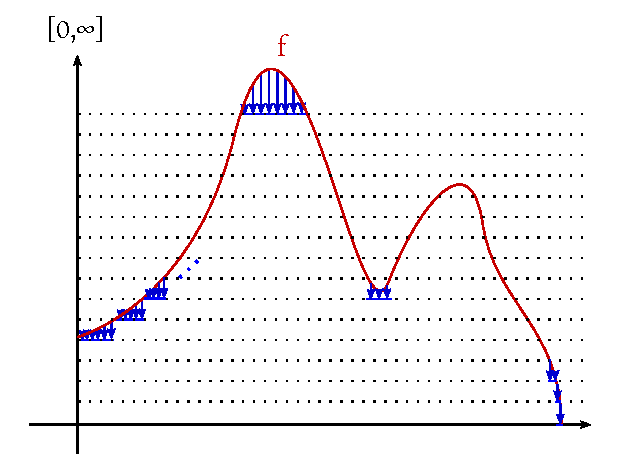
\includegraphics{img/02_lebesgue_integral.pdf}
          \caption{Illustration of the lebesgue integral}
          \label{img:lebesgue}
        \end{center}
      \end{figure}

      Let $f_n, g_n$ be simple.
      $f_n + g_n \nearrow f + g$

      \[ \int (f + g) \, d\mu \overset{\text{monotonic convergence}}{=} \lim \int (f_n + g_n) \, d\mu \]
      \[ = \lim(\int f_n \, d\mu + \int g_n \, d\mu) \overset{\text{monotonic convergence}}{=} \int f \, d\mu + \int g \, d\mu \]
  \end{enumerate}
\end{proof}

Unlike the Riemann integral, we use horizontal lines instead of vertical lines.
Thus we partition the image, not the domain.

\section{Integrable functions}

\begin{definition}
  Let $f: (\chi, d) \to \overline{\mathbb R}$ is measurable.
  If not $\int f^+ \, d\mu = \int f^- \, d\mu = +\infty$,
  integral exists:
  \[ \int f \, d\mu = \int f^+ \, d\mu - \int f^- \, d\mu \]
  \[ f^+ = \max\Set{f, 0} \qquad f^- = \max\Set{-f, 0} \qquad f = f^+ - f^- \qquad \Abs{f} = f^+ + f^- \]
  $f$ is called integrable, if $\int f^+ \, d\mu < \infty$ and $\int f^- \, d\mu < \infty$
  \[ \iff \int f \, d\mu \text{ exists and is finite} \]
\end{definition}

\begin{remark}[Properties]\hfill
  \begin{enumerate}
    \item $f$ is integrable $\iff \Abs{f}$ is integrable and $\Abs{\int f \, d\mu} \leq \int \Abs{f} \, d\mu$
    \item $f$, $g$ are integrable with $f \leq g$ almost everywhere wrt. $\mu$ $\implies \int f \, d\mu \leq \int g \, d\mu$
    \item $f$ is integrable, $\alpha \in \mathbb R \implies \alpha \cdot f$ is integrable and $\int (\alpha \cdot f) \, d\mu = \alpha \cdot \int f \, d\mu$
    \item $f, g$ are integrable $\implies f + g$ is integrable and $\int (f + g) \, d\mu = \int f \, d\mu + \int g \, d\mu$
  \end{enumerate}
\end{remark}

% We defined $0 \cdot \infty = 0$.  % this property is not necessary for the proof

\begin{proof}
  \begin{enumerate}
    \item $f$ is integrable
      \[ :\iff \int f^{\pm} \, d\mu < \infty \iff \underbrace{\int f^+ \, d\mu + \int f^- \, d\mu < \infty}_{\int \Abs{f} \, d\mu < \infty} \]
      \begin{align*}
        \Abs{\int f \, d\mu} &= \Abs{\int f^+ \, d\mu - \int f^- \, d\mu} \\
          &\leq \int f^+ \, d\mu + \int f^- \, d\mu \\
          &= \int \Abs{f} \, d\mu
      \end{align*}
    \item $f^+ - f^- \overset{\substack{\text{almost} \\ \text{everywhere}}}{\leq} g^+ - g^- \implies f^+ + g^- \overset{\text{a.e.}}{\leq} f^- + g^+$
      \[ \int f^+ \, d\mu + \int g^- \, d\mu = \int (f^+ + g^-) \, d\mu \leq \int \left(f^- + g^+\right) \, d\mu = \int f^- \, d\mu + \int g^+ \, d\mu \]
      \[ \int f^+ \, d\mu - \int f^- \, d\mu \leq \int g^+ \, d\mu - \int g^- \, d\mu \]
      It is important to recognize that all integrals are finite.
    \item For $\alpha = 0$, the statement is true. Consider $\alpha > 0$.
      \[ (\alpha f)^{\pm} = \alpha \cdot f^{\pm} \qquad \int \alpha f \, d\mu = \int \alpha \cdot f^+ \, d\mu - \int \alpha \cdot f^- \, d\mu = \alpha \int f^+ \, d\mu - \alpha \int f^- \, d\mu \]
      Now consider $\alpha < 0$, or more simply $\alpha = -1$ (any negative number is the product of a positive number and $-1$):
      \[ (-f)^+ = f^- (-f)^- = f^+ \qquad \dots \]
    \item $(f + g)^+ - (f + g)^- = f + g = f^+ + g^+ - (f^- + g^-)$
      \[ (f + g)^+ + f^- + g^- = (f + g)^- + f^+ + g^+ \]
      \[ \int (f + g)^+ \, d\mu + \int f^- \, d\mu + \int g^- \, d\mu = \int (f + g)^- \, d\mu + \int f^+ \, d\mu + \int g^+ \, d\mu \]
      \[ \int (f + g)^+ \, d\mu - \int (f + g)^- \, d\mu = \int f^+ \, d\mu - \int f^- \, d\mu + \int g^+ \, d\mu - \int g^- \, d\mu \]
  \end{enumerate}
\end{proof}

Riemann integral only works for $\mathbb R^n$.
The Lebesgue integral works for any measure space.

\begin{example}
  We consider the Riemann integral:
  \[ \pi = \int_{-\infty}^\infty \frac{\sin{x}}{x} \, dx \overset{\text{Riemann}}{=} \lim_{c,d\to \infty} \int_{-c}^d \frac{\sin{x}}{x} \, dx \text{ exists} \]
  If you consider $\frac{\sin{x}}{x}$ for one $\pi$, we have a positive and negative area.
  By Leibniz criterion, we have an alternating series and its limit is zero.

  We consider the Lebesgue integral:
  \[ \int_{\mathbb R} \Abs{\frac{\sin{x}}{x}} \, dx = +\infty \]
  $\frac{\sin{x}}{x}$ is not Lebesgue-integrable.
  Because in case of the Lebesgue integral, we don't consider an alternating series, but need to consider $\Abs{f}$, which is non-negative and the series does not converge.
\end{example}

\begin{theorem}[Dominated convergence theorem by Lebesgue]
  Let $f_n: (\chi, \mathcal A) \to \overline{\mathbb R}$ be a sequence of measurable functions.
  $f_n \to f$ pointwise [almost everywhere wrt. $\mu$]. There exists $g: (\chi, \mathcal A) \to [0, \infty]$ integrable [$\int g \, d\mu < \infty$].
  \[ \Abs{f_n} \leq g \text{ almost everywhere wrt. } \mu \forall n \implies \int f \, d\mu = \lim_{n\to\infty} \int f_n \, d\mu \]
\end{theorem}

\begin{proof}
  Without loss of generality, almost everywhere implies everywhere.

  \[ \Abs{f} = \lim{\Abs{f_n}} \leq g \qquad \text{ all of  them are integrable } \]
  \[ g_n = 2g - \Abs{f_n - f} \geq 0 \qquad g_n \to 2g \]
  \[ \liminf \int g_n \, d\mu \geq \int \left(\liminf g_n\right) \, d\mu \overset{g_n \to 2g}{=} \int \left(\lim g_n\right) \, d\mu = 2 \int g \, d\mu \]
  \[ \int g \, d\mu - \limsup \int \Abs{f_n - f} \, d\mu = \liminf \int g_n \, d\mu = 2\int g \, d\mu \]
  \[ \limsup\Abs{\int f_n \, d\mu - \int f \, d\mu} \leq \limsup \int \Abs{f_n - f} \, d\mu = 0 \]

  Again:
  \[ \int g_n = \left(\int 2g - \int \Abs{f_n - f}\right) \]
  \[ \implies \limsup \int g_n = \limsup \left(\int 2g - \int \Abs{f_n - f}\right) \]
  \[ = \int 2g + \limsup \left(-\int \Abs{f_n - f}\right) = \int 2g - \liminf \left(\int \Abs{f_n - f}\right) \]
\end{proof}

\dateref{2018/11/05}

\begin{Remark}[Dominated convergence theorem by Lebesgue]
  $f_n, f, g: (\chi, \mathcal A, \mu) \to (\mathbb R, \mathcal B_{\overline{\mathbb R}}$.
  \[ \begin{cases} f_n \to f & \mu \text{ almost everywhere} \\ \Norm{f_n} \leq g & \mu \text{ almost everywhere} \end{cases} g \geq 0, \int_{\chi} g \, d\mu < \infty \]
  \[ \implies \int {\chi} f \, dx = \lim_{n\to\infty} \int_{\chi} f_n \, d\mu \]
\end{Remark}

\begin{example}
  $([0, 1], \mathcal B_{[0,1]}, \lambda)$ with $f_n(x) \to 0$ and $\int_{[0,1]} f_n \, d\lambda = 1 \centernot{\implies} \int_{[0,1]} 0 \, d\mu$.
  Compare with Figure~\ref{img:exconv}.

  \begin{figure}
    \begin{center}
      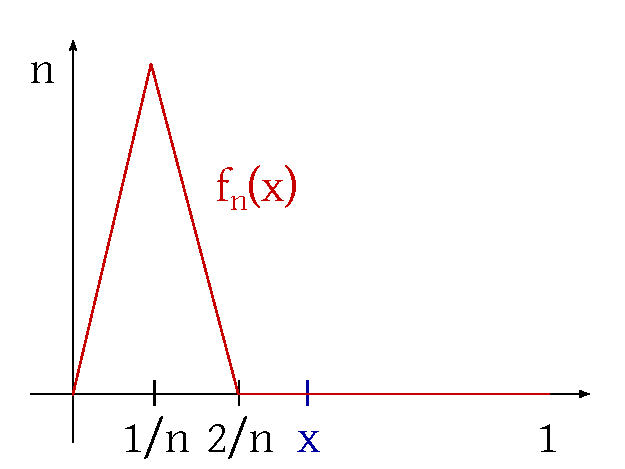
\includegraphics{img/03_convergence.pdf}
      \caption{$f_n(x)$}
      \label{img:exconv}
    \end{center}
  \end{figure}
\end{example}

The theorem of convergence is a generalization of the following theorem (based on Analysis 1 and Analysis 2 courses):

\begin{example}[Monotonic convergence]
  \[ f(x) = \sum_{n=0}^\infty a_n x^n \qquad a_n \geq 0 \]
  Convergence raidus: $R < \infty$.
  \[ x_k \nearrow R \implies f_k(x) \nearrow f(R) \]
  \[ \chi = \mathbb N_0, \mathcal A = \mathcal P(\mathbb N_0), \mu \]
  \enquote{counting measure}
  \[ f_k(n) = a_n x_k^n \]

  \[ f: \mathbb N_0 \to [0, \infty] \]
  \[ \int_{\mathbb N_0} f \, d\mu = \sum_{n=0}^\infty f(n) \mu(n) \]
  for $k \to \infty$: $f_k(n) \nearrow f(n) = a_n R^n$.
  By monontonic convergence, $\int f_k \, d\mu \nearrow \int f \, d\mu$.
  \[ \sum_{n=0}^\infty a_n x_k^n \nearrow \sum_{n=0}^\infty a_n R^n \]
\end{example}

\section{Lebesgue and Riemann integral}

$\lambda$ is defined on $(\overline{\mathbb R}, \mathcal B_{\overline{\mathbb R}})$.
The Lebesgue measure allows null sets. Lebesgue measure is also defined on completion of sigma algebras.
Lebesgue measure $\mathcal L$ is defined on $\sigma$-algebras of Lebesgue sets.

\begin{Remark}[One characterization of the Axiom of Choice]
  A non-empty product of non-empty sets is non-empty.
\end{Remark}
\begin{Remark}
  $\mathcal L \setminus \mathcal B \neq \emptyset$ [Axiom of Choice].
\end{Remark}

\begin{Remark}[Number representation]
  Basis $q \in \Set{2, 3, \dots}$.
  \[ x = \sum_{n=1}^\infty \frac{x_n}{q^n} \qquad x_n \in \Set{0,1,\dots,q-1} \]
  This represents a number $0 . x_1 x_2 x_3 x_4 \dots$.

  Because $0.7\overline{9} = 0.8$, there is some ambiguity between the numbers and their representation (non-bijective, two sums represent the same $x$).
\end{Remark}

\begin{Remark}[Cantor set]
  Consider $[0, 1]$. Split the interval into 3 thirds. We remove the middle third as open set.
  We consider the remaining two intervals and again extract the middle third.
  We iteratively continue this process to infinity.
  The remaining set is called Cantor set and is uncountable.

  The Cantor set $\mathcal C$ is the set of numbers in $[0,1]$ with some number representation, with respect to basis $3$, which does not contain some $1$ and has a unique number representation. Unique number representation because
  \[ \frac23 = 0.2 = 0.1\overline{2} \]
  \[ \frac13 = 0.1 = 0.0\overline{2} \qquad \frac19 = 0.01 = 0.00\overline{2} \qquad \frac29 = 0.02 = 0.01\overline{2} \]
\end{Remark}

A linear combination of Borel-measurable functions is Borel-measurable.

\begin{Remark}
  Riemann integral ($U$ are lower sums, $O$ are upper sums):
  \[ f: [a,b] \to \mathbb R \text{ bounded} \]
  \[ Z = \Set{a = x_0 < x_1 < \dots < x_k = b} \qquad \Norm{Z} = \max_{j=1,k} (x_j - x_{j-1}) \]
  \[ m_j = \inf_{x \in [x_{j-1}, x_j]} f(x) \qquad M_j = \sup_{x \in [x_{j-1}, x_j]} f(x) \]

  \[ U(Z, f) = \sum_{j=1}^k m_j(x_j - x_{j-1}) \]
  \[ g_Z = \sum_{j=1}^k m_j \mathbf{1}_{(x_{j-1}, x_j]} \text{ are both } \mathcal B\text{-measurable} \]
  \[ U(Z, f) = \sum_{j=1}^l M_j (x_j - x_{j-1}) \]
  \[ h_Z = \sum_{j=1}^k M_j \mathbf{1}_{(x_{j-1}, x_j]} \]
  \[ U(Z, f) = \int_{[a,b]} g_Z \, d\lambda \qquad O(Z, f) = \int_{[a,b]} h_Z \, d\lambda \]
\end{Remark}

\begin{theorem}
  $f$ as above (if necessary, not Borel-measurable)
  \[ C = \Set{x \in [a,b]: f \text{ continuous in } x} \quad D = \SetDef{x \in [a,b]}{f \text{ in } x \text{ is non-continuous}} \]
  \begin{enumerate}
    \item Then $C, D \in \mathcal B_{[a,b]}$, $f \cdot \mathbf{1}_C$ is Borel-measurable
    \item $f$ is Riemann integrable $\iff \lambda(D) = 0$ and
      \[ \int_a^b f(x) \, dx = \int_{[a,b]} f \cdot \mathbf{1}_C \, d\lambda \]
  \end{enumerate}
\end{theorem}

\begin{proof}
  \[ Z_n = \Set{a = x_0^{(n)} < x_1^{(n)} < \dots < x_{k(n)}^{(n)} = b} \]
  A sequence of decompositions such that
  \begin{enumerate}
    \item $Z_{n+1}$ is refinement of $Z_n$
    \item $\Norm{Z_n} \to 0$
  \end{enumerate}
  except for point $a$ (so the intervals are left-sided half-open) (you can also close the first interval of the left side)
  \[ \inf{f} = m \leq g_{Z_n} \nearrow g \leq f \leq h \swarrow h_{Z_n} \leq M = \sup{f} \]
  where $g$ and $h$ are Borel-measurable. By the dominated convergence theorem by Lebesgue,
  \[ U(Z_n, f) = \int_{[a,b]} g_{Z_n} \, d\lambda \nearrow \int_{[a,b]} g \, d\lambda \]
  \[ O(Z_n, f) = \int h_{Z_n} \, d\lambda \searrow \int_{[a,b]} h \, d\lambda \]
  $R = \SetDef{x_j^{(n)}}{n \in \mathbb N, j = 1, \dots, k(n)}$ is countable, $\lambda(R) = 0$.
\end{proof}

\begin{claim}
  For $x \in [a,b] \setminus R$, $f$ is continuous at $x \iff g(x) = h(x)$.
\end{claim}

\begin{proof}
  Let $I_n(x)$ be the interval of $Z_n$ with $x \in I_n(x)$.
  Recognize that $I_{n+1}(x) \subset I_n(x)$ and $\lambda(I_n(x)) \searrow 0$.

  \begin{align*}
    f \text{ cont. in } x
      &\iff \forall \varepsilon > 0 \exists k: f(x) - \varepsilon < f_{I_k(x)} < f(x) + \varepsilon \\
      &\iff \forall \varepsilon > 0 \forall n \geq k: f(x) - \varepsilon < f_{I_k(x)} < f(x) + \varepsilon \\
      &\iff \forall \varepsilon > 0 \exists k \forall n \geq k: f(x) - \varepsilon \leq \left. g_{Z_1} \right|_{I_n(x)} \leq \left. h_{Z_n} \right|_{I_n(x)} \leq f(x) + \varepsilon \\
      &\Rightarrow g(x) = h(x) \qquad [= f(x)]
  \end{align*}
  \enquote{$\Rightarrow$} is \enquote{$\iff$} assuming $x \not\in R$,
  so $[g < h] \subset D \subset [g < h] \cup R$ where $[g < h]$ is the Borel set.
  \[ D \setminus [g < h] \text{ is at most countable (because $R$ is countable)} \implies D \text{ Borel set}, C \text{ Borel set} \]
  \[ \lambda(D) = \lambda[g < h] \]
\end{proof}

\[ f \text{ is R-integrable } \iff \int_{[a,b]} g \, d\lambda = \int_{[a,b]} h \, d\lambda, h \geq g \]
\[ \iff \lambda[g < h] = 0 \iff \lambda(D) = 0 \]
in this case (because $g \leq f \leq h$ except in $a$).
\[ g \cdot \mathbf{1}_C = f \cdot \mathbf{1}_C \]
where $g$ and $\mathbf{1}_C$ is Borel-measurable and thus $f \cdot \mathbf{1}_C$ is Borel-measurable.
\[ \int_{[a,b]} f \cdot \mathbf{1}_C \, d\lambda = \int_{[a,b]} g \cdot \mathbf{1}_C \, d\lambda = \int_{[a,b]} g \, d\lambda = \int_a^b f(x) \, dx \]
\[ g \cdot \mathbf{1}_C = g \qquad \text{ almost everywhere wrt. } \lambda \]

\begin{example}
  \begin{enumerate}
    \item $\mathbf{1}_{\mathbb Q}$ is nowhere continuous.
      \[ \int_0^1 \mathbf{1}_{\mathbb Q}(x) \, dx \text{ does not exist} \]
      \[ \mathbf{1}_{\mathbb Q} = 0 \qquad \text{ almost everywhere wrt. } \lambda \implies \int_{[0,1]} \mathbf{1}_{\mathbb Q} \, d\lambda = 0 \]
    \item
      \[ \int_a^b \frac{\sin{x}}{x} \, dx = \int_{[a,b]} \frac{\sin{x}}{x} \, dx \]
      \[ \int_{-\infty}^\infty \frac{\sin{x}}{x} \, dx = \pi \qquad \not\exists \int_{\mathbb R} \frac{\sin{x}}{x} \, d\lambda(x) \]
  \end{enumerate}
\end{example}

\begin{theorem}[Substitution theorem]
  Let $\varphi: (\chi, \mathbb A, \mu) \to (\chi', \mathcal A')$ is measurable.
  \[ \mu_{\varphi}(A') = \mu(\varphi^{-1}(A')) \qquad A' \in \mathcal A' \qquad \text{ pushforward measure} \]
  \[ f: (\chi', \mathcal A') \to (\overline{\mathbb R}, \mathcal B_{\overline{\mathbb R}}) \text{ measurable} \]
  Then,
  \[ \int_{\chi} f \circ \varphi \, d\mu \text{ exists } \iff \int_{\chi'} f \, d\mu_{\varphi} \text{ exists} \]
  and in this case, they are the same.
\end{theorem}

\printindex

\end{document}
